% !TEX root = ../main.tex
%
\chapter{Related Work}
\label{sec:related}

% Overview (free-by-me) READY
Before describing the problem, and later on the experimental setup, we first
\begin{enumerate}
    \item Revise three common prediction tasks in \acp{gnn}
    \item Give a general overview of how \acp{gnn} organize and process graph structured data
    \item We further discuss the relation of messasge passing mechanis to the \ac{wl}, an algorithm for
          inspecting wheather two graphs are isomorph.
    \item Give an formal definition and description of two \ac{gnn}
          architectures, which will be used in our experiments.
\end{enumerate}


\section{Prediction Tasks and Typical Problems}
\label{sec:related:pred}

% Types of prediction tasks (free-by-me) READY
Graphs naturally appear in numerous application domains, ranging from social analysis,
bioinformatics to computer vision.
A Graph $G = (V,E)$, where $V = \{v_{1},...,v_{n}\}$ is a set of $N =|V|$ nodes and
$E \subseteq V\times V$ a set of edges betwen those nodes. The unique capability of
graphs enables capturing the structural relations among data, and thus allows to harvest more
insights compared to analyzing data in isolation~\cite{Zhang19}. Graphs therefore can be
seen as a general laguage for describing entities and relationships between those entities.
\Acfp{gnn} then organize graph structured data to tackle various prediction and classification
tasks. Typically, one is interested in one of the following three tasks:
\begin{enumerate}[label=\textbf{\arabic*.}]
    \item \textbf{Link prediction:}
          Predict whether there are missing links between two nodes
          e.g., knowledge graph completion

    \item \textbf{Vertex classification \& regression:}
          Predict a property of a node e.g., categorize online users/items

    \item \textbf{Graph classification \& regression:}
          Here we are interested in classifying or predicting a continous value for
          the entire graph e.g., predicting a property of a molecule.
\end{enumerate}

In this work the main focus will be on the latter two, \ac{nc}\ \ac{nr} and \ac{gc}\
\ac{gr} for small- as well as large-sized graphs.

% Message passing formally
\section{Passing Messages in \Acsp*{gnn}}
\label{sec:related:message}

% Intro to GNNs, State-description (free-by-me) READY
Graphs, by nature are unstructured. Vertices in graphs have no natural order and can
contatin any type of information. In order for machine learning algorithms to be able
to make use of graph structured data, a mechanism is needed to organize them in a
suitable way~\cite{Zhou2020a,Hamilton2017a,Zhang19}.


% Message Passing in general (free-by-me) READY
Message passing is a mechanism~\cite{Xu2019,Zhou2020a}, which embedds into every node information about it's neighbourhood.
This can be done in several ways and one way of classifying a \ac{gnn} is by looking at the
underlying message passing machanism. In this paper we will look at a network, where message passing is done
via convolutions (\acf{gcn}). We will however ocasionally use the more general term message passing, as
the separation is rather blurred and message passing describes a neighborhood aggregation scheme and
is seen as a generalization of other, more specific mechanisms.

Formally, message passing in a \ac{gnn} can be described as using two functions:
AGGREGATE and COMBINE. The expressive and representational power of a \ac{gnn} can
then be determined by looking at the concrete functions and thier properties, used to implement
aggregation and combination. AGGREGATE mixes in every iteration the hidden representation of the node
with the representation of nodes neighbourhood. COMBINE then combines the mixed representation togheter with the
representation of the node. Each node uses the information from its neighbors to update its embeddings, thus a natural
extension is to use the information to increase the receptive field by performing AGGREGATE and COMBINE multiple
times.

\begin{align*}
    a_{v}^{k} = \mathrm{AGGREGATE}^{(k)}(\{h_{u}^{(k-1)}: u \in \mathcal{N}_{(v)}\}) , h_{v}^{(k)} = \mathrm{COMBINE}^{(k)}(h_{v}^{(k-1)}, a_{v}^{(k)})
\end{align*}

For graph-level predictions an additional READOUT- operation is used:
\begin{align*}
    h_{G} =\mathrm{READOUT}(\{h_{v}^{(K)}| v \in G\})
\end{align*}

% Message passing framework and local graph structure (free-by-me) READY
One useful type of information, which the message passing framework should be able to
capture, is the local graph structure. This can be done by choosing functions with
appropriate properties. A more detailed explanation will follow in
\cref{sec:related:architectures}. In spatial \ac{gnn} we make the assumption of the
similarity of neighbor nodes. To exploit this spatial similarity, we perform
composition by stacking multiple layers togheter and increase the receptive field.

% picture of k-hop neighbourhood aggregation (free-by-me) READY
\begin{figure}[ht]
    \centering
    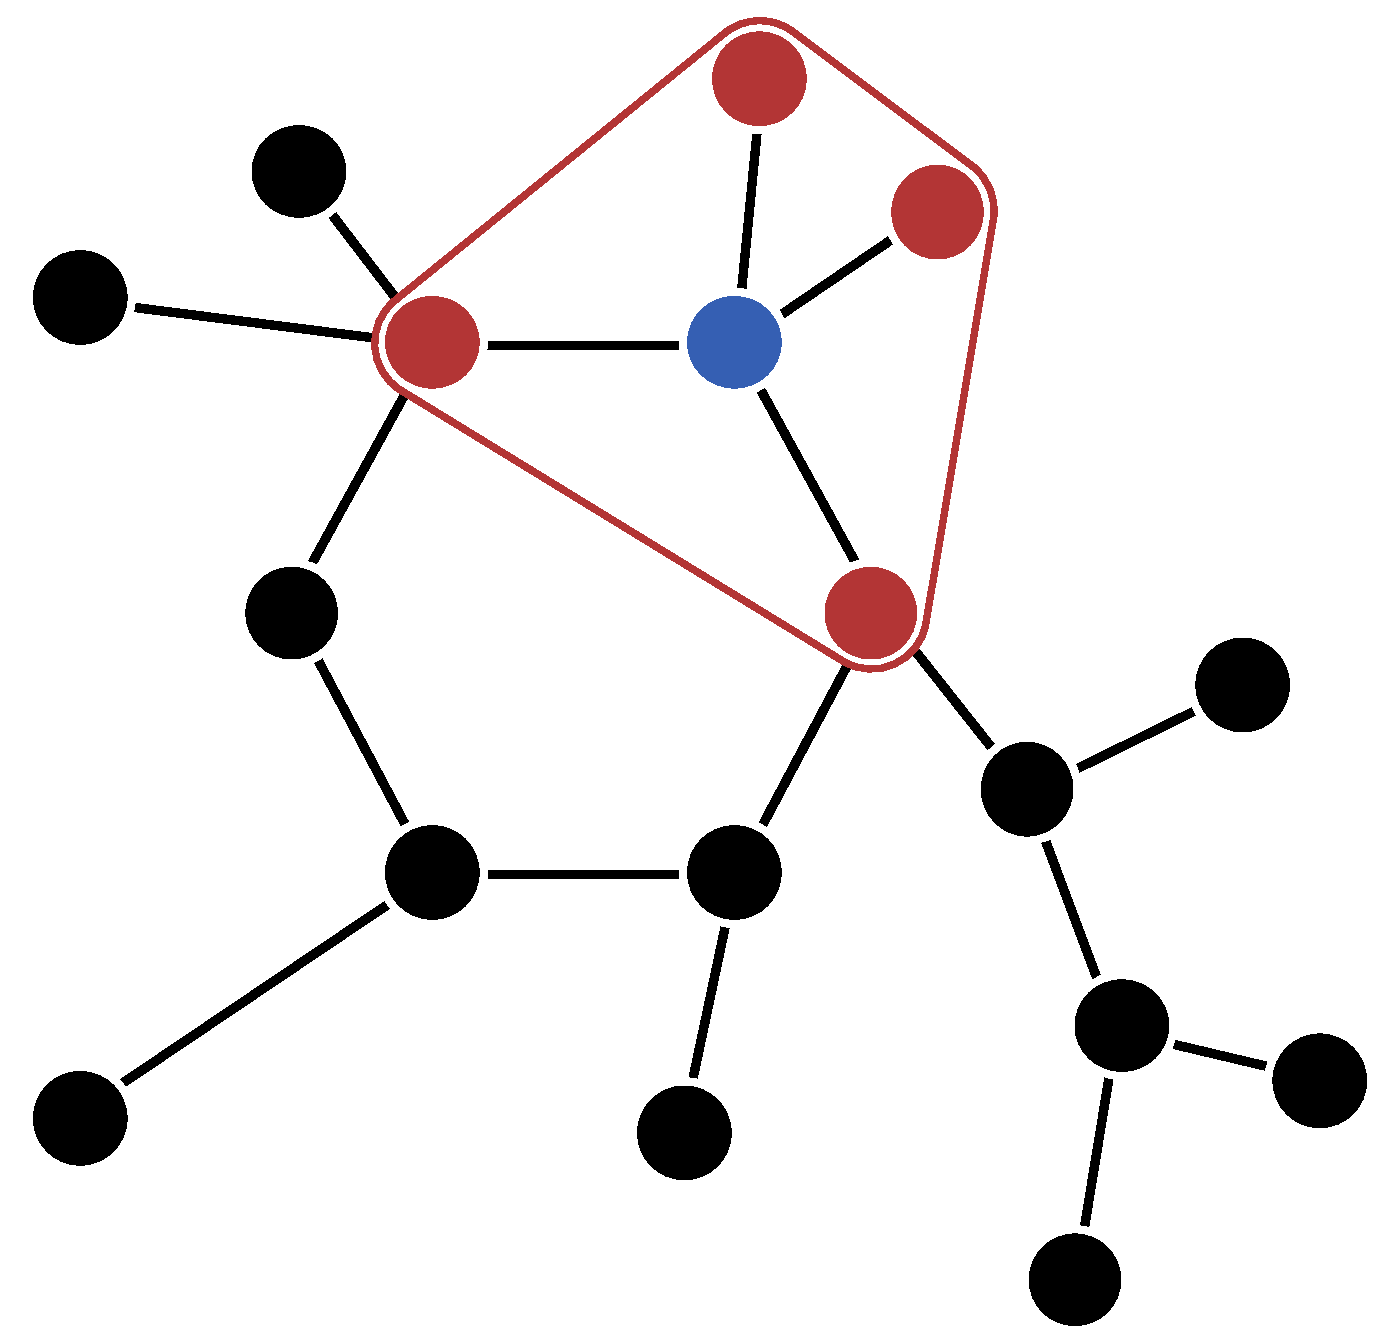
\includegraphics[width=0.35\linewidth]{gfx/related-work/1hop}\hspace{1cm}
    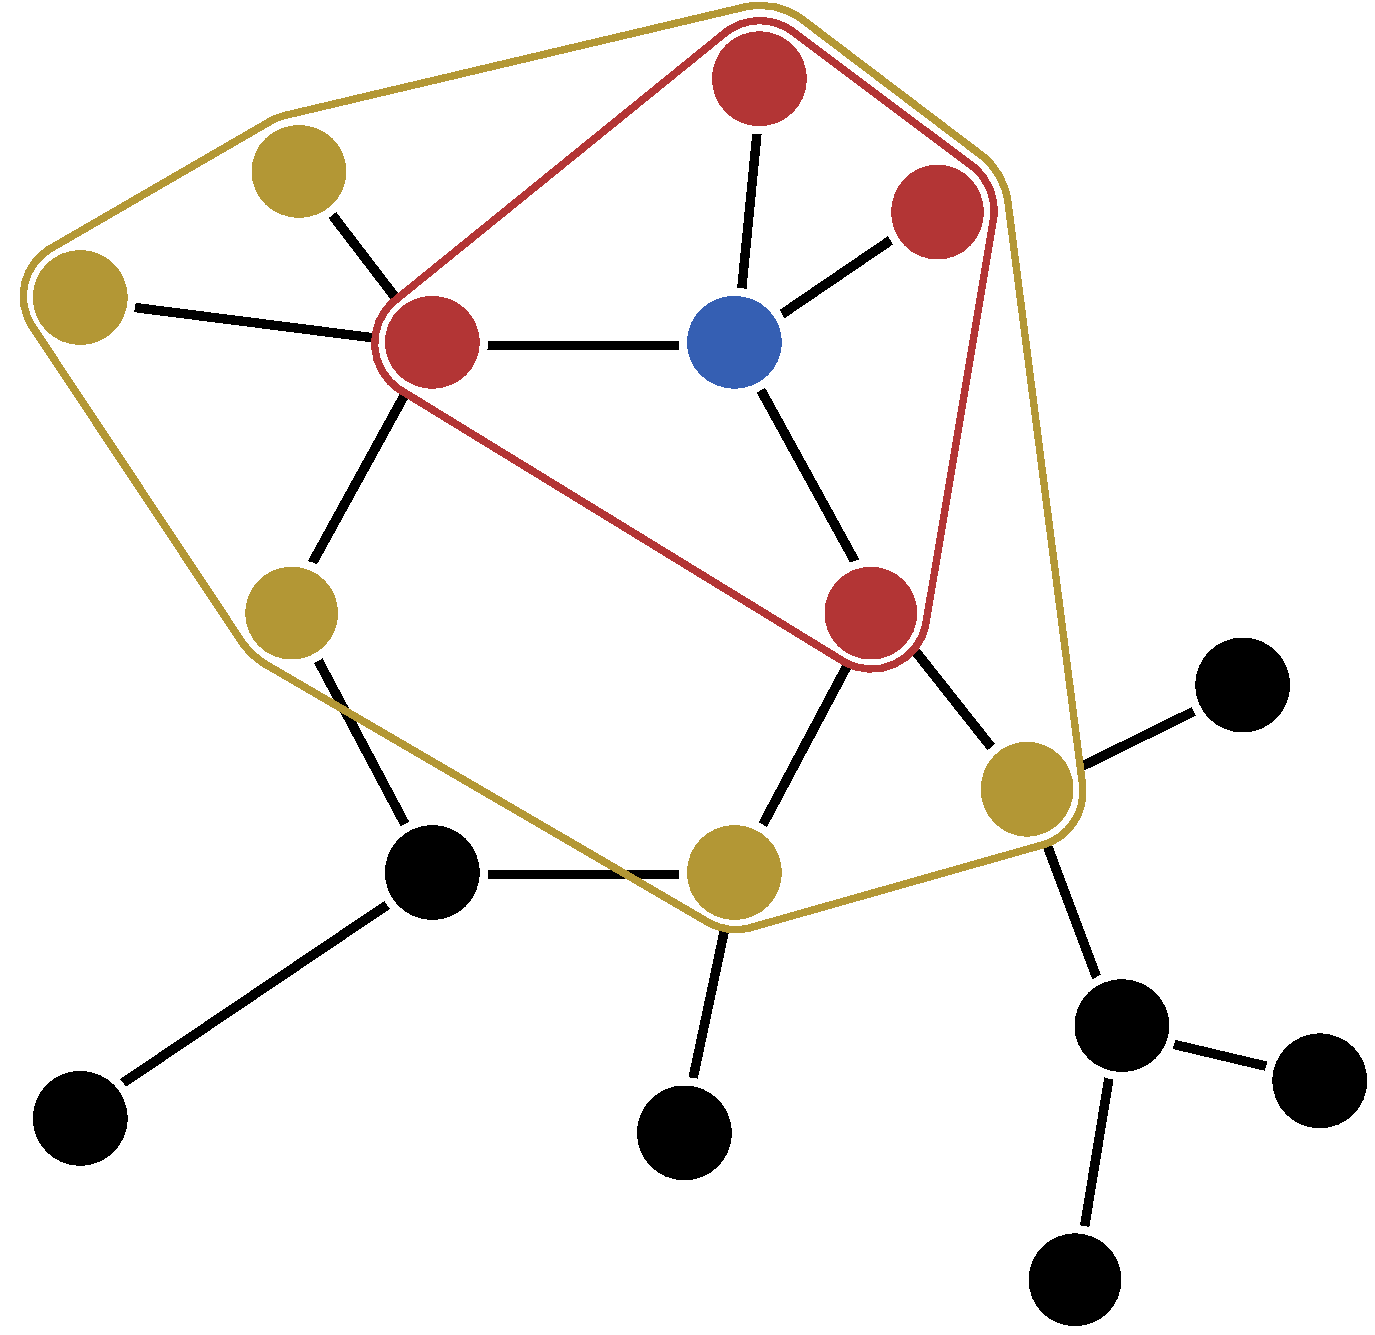
\includegraphics[width=0.35\linewidth]{gfx/related-work/2hop}
    \caption{By performing aggregation k-times we can reach and capture the
        structural information of the k-hop neighborhood}\label{fig:related:1hop}
\end{figure}


\subsection{\acl{wl} Graph Colorings}
\label{sec:related:character:wl}
% What is the Weisfeiler lehman test 
% Definition and relation to neural networks (free-by-me) READY
The Message passing mechanism has a close relation, to the way the \acf{wl} test ~\cite{Weisfeiler1968}
~\cite{Damke2020}~\cite{Huang2022}, an algorithm for deciding wheather two graphs are isomorphic works.
Before describing the algorithm, we introduce notations and preliminaries.\\
% Intro of Notations 
%---------------
% Table 
%---------------
% Graph definition --> Your neighbors are communicating 
Let $G = (V,E, X)$ denote an undirected graph where $V =\{v_{1},...,v_{n}\}$ is a set of $ N = |V|$
nodes and $E \subseteq V\times V $ a set of edges between those nodes. For simplicity we
represent an edge ${v,u}$ by $(v,u) \in E$ or $(u,v)$.$X= [x_{1},...,x_{n}]^{T} \in \mathbb{R}^{n \times d}$
is the node feature matrix, where $n = |V|$ is the number of nodes and $x_{v} \in \mathbb{R}^{d}$
represents the \textit{d}-dimensional feature of node $v$. $\mathcal{N}_{v}= \{u \in V|(v,u) \in E\}$
is the set of neighboring nodes of node $v$. A multiset is denoted
as $\ldblbrace...\rdblbrace$ and formally defined as follows.
% Multiset --> Your neighbors are communicating 
\begin{defn}[Multiset]
    A multiset is a generalized concept of set allowing repeating elements. A multiset $X$
    can be formally represented by a 2-tuple as $X = (S_{X}, m_{X})$, where $S_{X}$ is the
    underlying set formed by the distinct elements in the multiset and $m_{X}:S_{X} \rightarrow
        \mathbb{Z}^{+}$ gives the multiplicity (i.e, the number of occurrences) of the elements.
    If the elements in the multiset are generally drawn from a set $X$ (i.e., $S_{X} \subseteq X$),
    then $\mathcal{X}$ is the universe of X and we denote it as $X \subseteq \mathcal{X}$ for ease
    of notation.
\end{defn}
% Isomorphism --> Your neighbors are communicating 
\begin{defn}[Isomorphism]
    Two Graphs $\mathcal{G}= (V,E,X)$ and $\mathcal{H}= (P,F,Y)$ are \textit{isomorphic}, denoted as
    $\mathcal{G} \simeq \mathcal{H}$, if there exists a \textit{bijective} mapping $g: V \rightarrow P$
    such that $x_{v}= y_{g(v)}$, $\forall v \in V$ and $(v,u) \in E$ iff $(g(v),g(u)) \in F$. Graph
    Isomorphism is still an open problem without a known polynomial-time solution.
\end{defn}
% Define notations 



% The 1-WL in it's one-dimensional form (free-by-me) ok? 
\subsubsection{The 1-dimensional \acs{wl} algorithm (color refinement)}
In the 1-dimensional \ac{wl} algorithm (1-WL), a label, called color $c_{v}^{0}$ is assigned to each
vertex of a graph. Then, in every iteration the colors get updated based on the multiset representation
of the neighborhood of the node until convergence. If at some iteration the colorings of the graphs
differ, 1-\ac{wl} decides, that the graphs are not isorprphic.
\begin{align*}
    c_{v}^{l} \leftarrow \mathrm{HASH}(c_{v}^{l-1}, \ldblbrace c_{u}^(l-1)| u \in \mathcal{N}_{v} \rdblbrace)
\end{align*}

Algorithmically this can be expressed as follows:
% 1-WL algorithm 
\begin{algorithm}
    \caption{1-dim.\ \ac{wl} (color refinement)}
    \begin{algorithmic}[1]
        \Require $G = (V,E,X_{V})$
        \State $c_{v}^{0} \gets \mathit{hash}(X_{v})$ for all $v \in V$
        \Repeat
        \State $c_{v}^{l} \gets \mathit{hash}(c_{v}^{l-1}, \ldblbrace c_{w}^{l-1}: w \in \mathcal N_{G}(v)\rdblbrace)$ forall $v \in V$
        \Until{$(c_{v}^l)_{v \in V} = (c_{v}^{l-1})_{v \in V}$}
        \State \Return $\ldblbrace c_{v}^l : v \in V \rdblbrace$
    \end{algorithmic}
\end{algorithm}

The 1-\ac{wl} is a heuristic method, which can efficiently distinguish a broad class of non-isomorphic
graphs~\cite{Babai1979}.
However there exist some corner cases, where the algorithm fails to classify
simple shapes as non-isomorphic.

% graphics isomorpc - distinguishable 
\begin{figure}[ht]
    \centering
    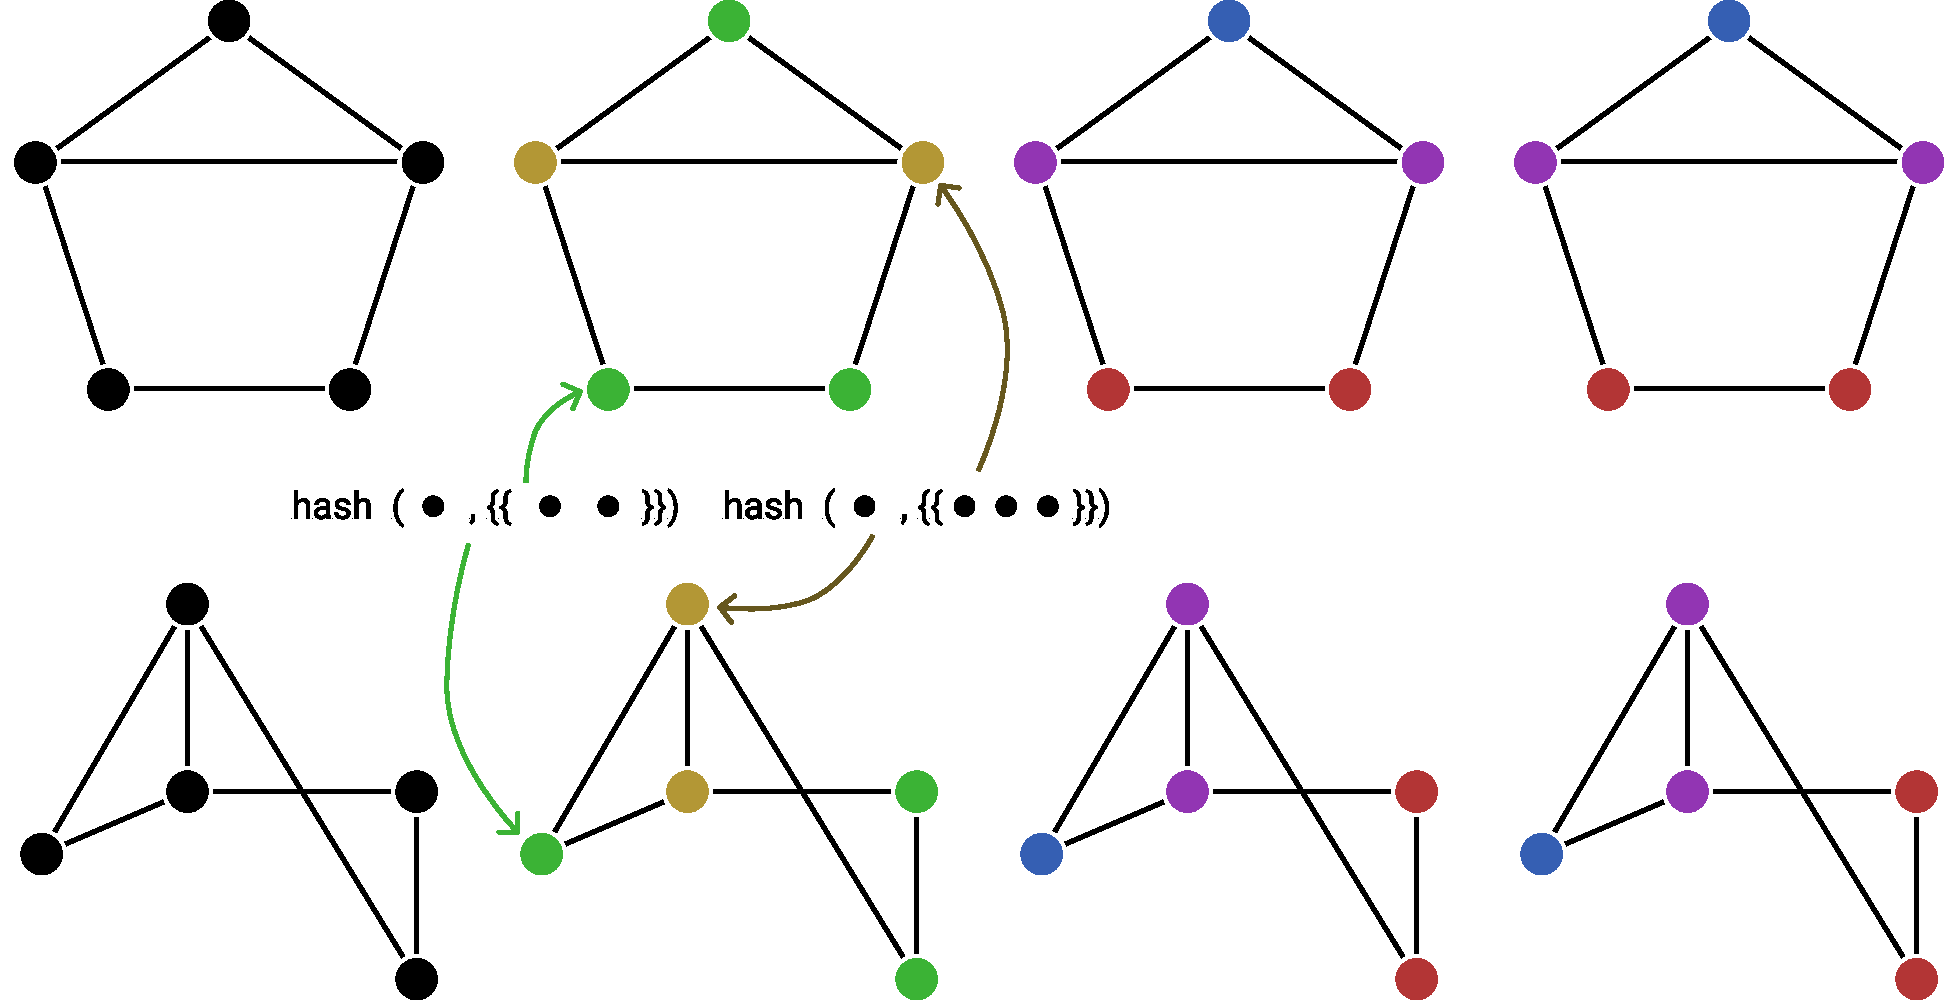
\includegraphics[width= 0.90\linewidth]{gfx/related-work/1wl-isomorph}
    \caption{1-\ac{wl}Two isomorphic graphs. 1-\ac{wl}assigns same
        representation}\label{fig:related:1-wl-indistinguishable}
\end{figure}

% graphics isomorpc - indistinguishable 
\begin{figure}[ht]
    \centering
    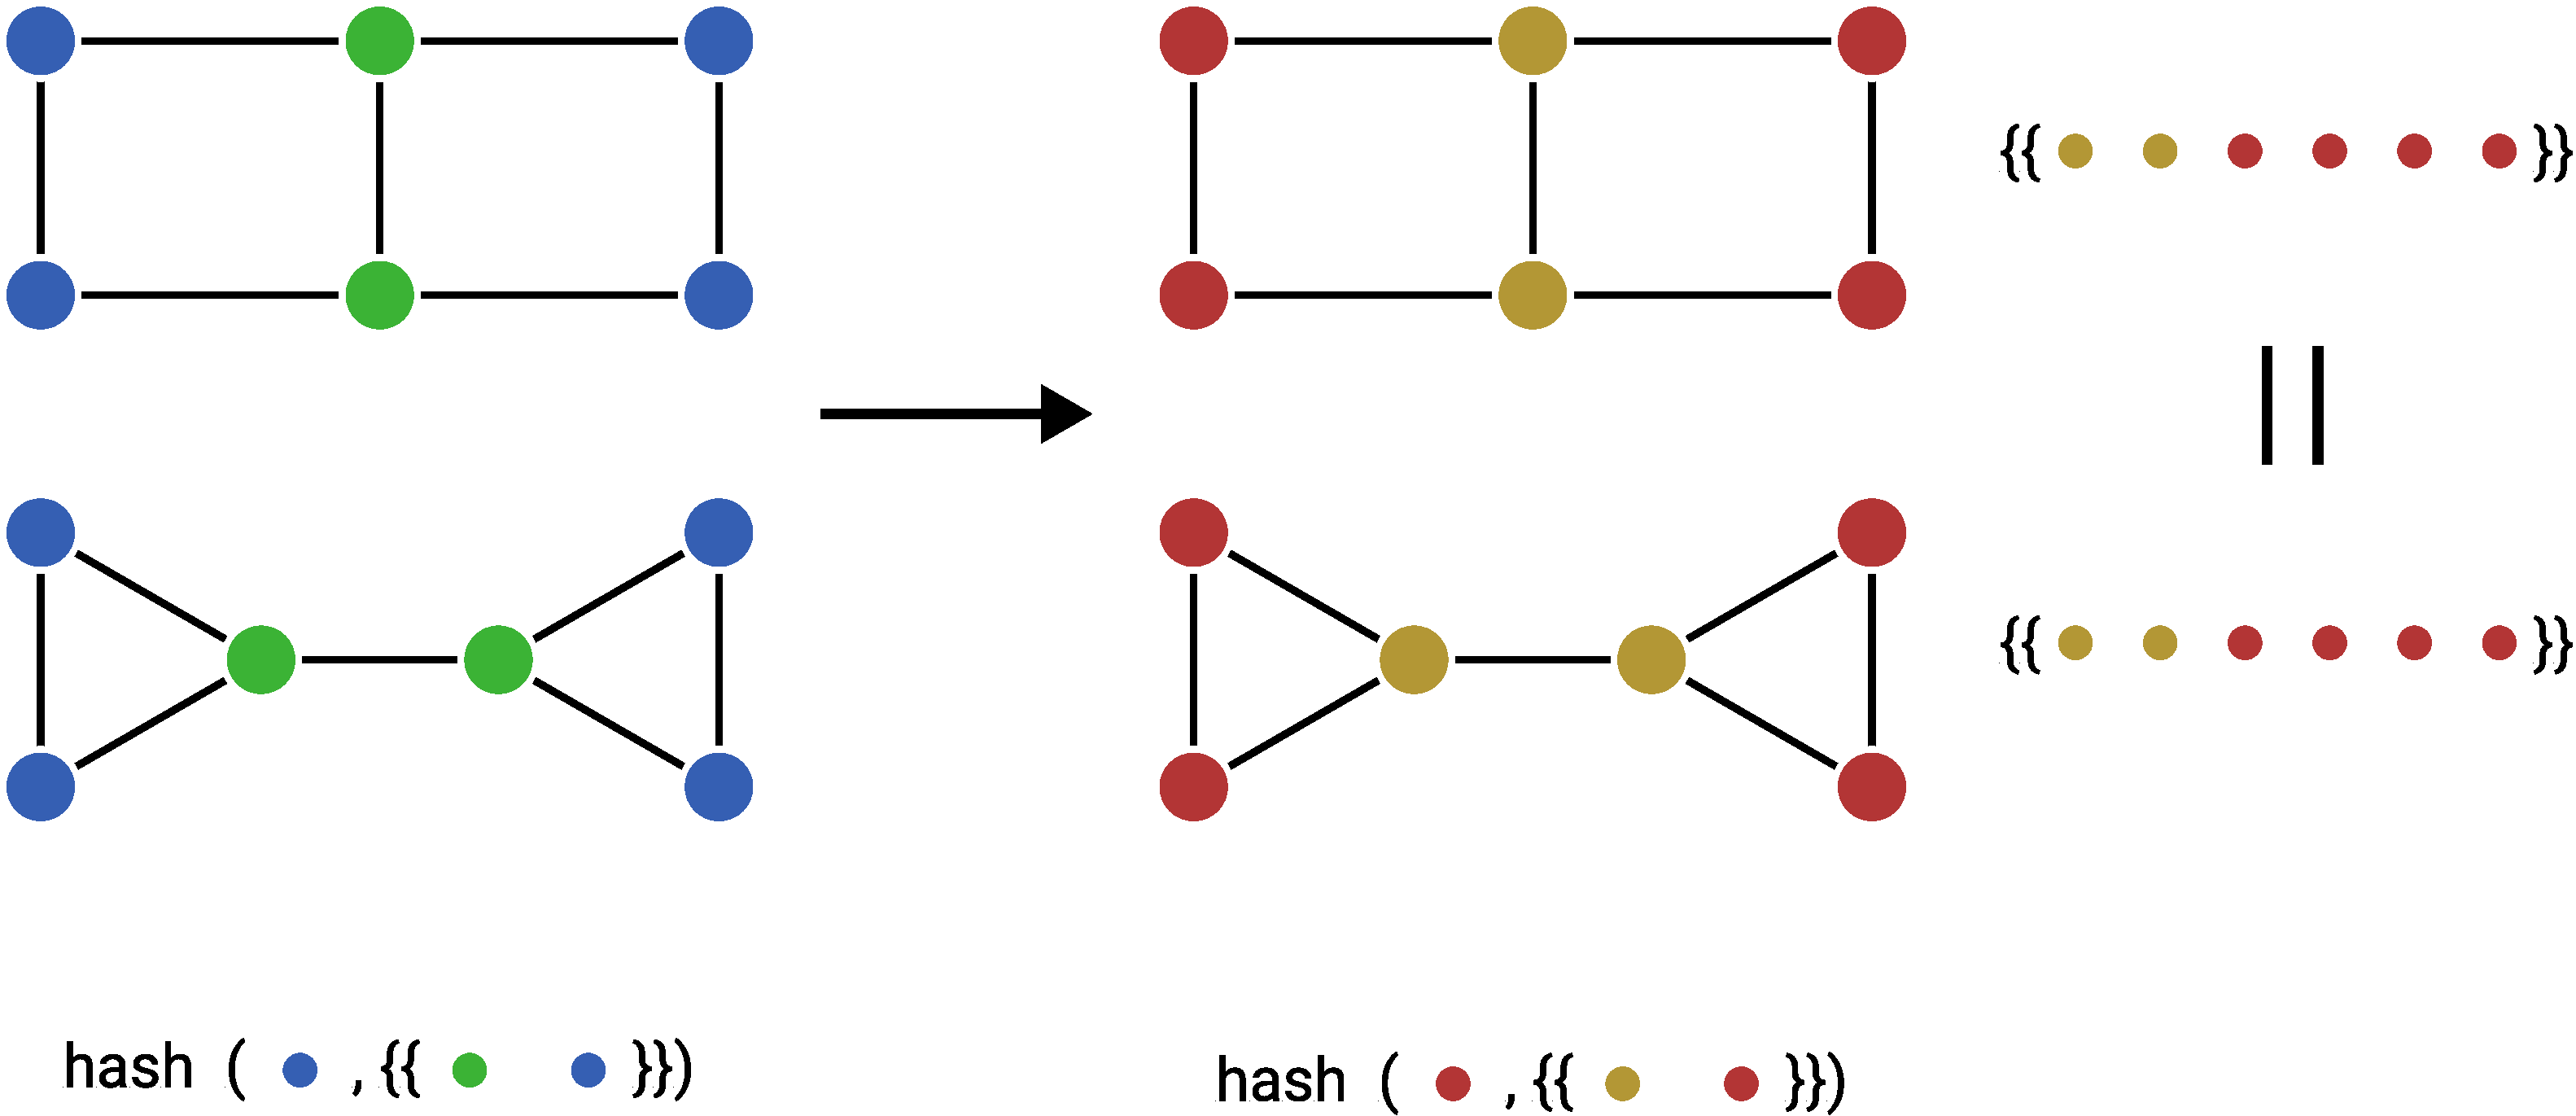
\includegraphics[width= 0.90\linewidth]{gfx/related-work/1wl-indistinguishable}
    \caption{1-\ac{wl} assigned one and the same labeling to two non-isomorphic graphs~\cite{Liu2022}}\label{fig:related:1-wl-indistinguishable}
\end{figure}


\subsection{GNN Architectures in this Paper}
\label{sec:related:architectures}

% Intro and motivation of the choice 
% Exploration of important properties 
% Where those networks achieve state of the art results 

% --> Convolutional network --> Image Processing 
% --> GIN, a powerful architecture ---> ecpecially in: 
% Motivation in Conclusion  
In the following section we briefly introduce and
motivate the choice of two types of networks, which we have
chosen to experiementally verify the efficacy of several regularization techniques, which will be
discussed in section \cref{sec:related:pred:regularization}.

% Explain why these architectures are a promising choice 
Since all of \ac{gnn} encorporate meaasge passing in a way, we decided to chose two interesting
architectures for our experiments, which in our view are promising.
\subsubsection{Graph Convolutional Network (GCN)}
\label{sec:related:architectures:gcn}
% History and Motivation 
Graph Convolutional Network \ac{gcn} was originally proposed by \citet{Kipf2017} to tackle
the problem of semi-supervised node classification, where lables are available for a small subset of
nodes. \ac{gnn}is a simple, but powerful architecture, that scales linearly in the number of graph
edges and learns hidden layer representations that encode both local graph structure and features of nodes.

% How does it operate formally 
A \acf{gcn} can formally be expressed via the following layer-wise propagation rule:

\begin{align*}
    H^{(l+1)} = \sigma (\tilde{D}^{-\frac{1}{2}}\tilde{A}\tilde{D}^{-\frac{1}{2}} H^{(l)}W^{(l)})
\end{align*}
Where $\tilde{A} = A + I_{N}$ is the adjacency matrix of the undirected graph $\mathcal{G}$
with added self-connections. $I_{N}$ is the identity matrix. $\tilde{D}_{ii} = \sum_{j}\tilde{A}_{ij}$and
$W^{l}$ is a layer-specific trainable weight-matrix.$\sigma(\cdot)$ denotes an activation function, such
as $ReLU(\cdot) = max(0, \cdot)$. $ H^{l}\in  \mathbb^{N \times D}$ is the matrix of activations in the
$l^{\mathrm{th}}$ layer; $H^{0}= X$

% How does it operate intuition --> relation to implementation 
Because we consider every neighbor to be of equal importance and therefore normalization is accomplished
by dividing by the number of neighbours, one can view this operation as performing an element-wise
mean-pooling~\cite{Xu2019}.
\begin{align*}
    h_{v}^{(k)} = \mathrm{ReLU}(\mathrm{W} \cdot\mathrm{MEAN} \{h_{u}^{k-1},\ \forall{u} \in \mathcal{N}_{(v)} \cup \{v\}\})
\end{align*}
An application of a two-layer \ac{gcn} is given by:

\begin{align*}
    Z = f(X,A) = \mathrm{softmax} (\hat{A}\ \mathrm{ReLU}(\hat{A}XW^{0})W^{l})
\end{align*}

where $\hat{A} = \tilde{D}^{-\frac{1}{2}}\tilde{A}\tilde{D^{-\frac{1}{2}}}$
is calculated in a preprocessing step. The model uses a single weight matrix per layer and
deals with varying node degrees through an appropriate normalization of the adjacency matrix.
% Experimental results and where it was expecially useful and why 
This model consisted of a 2-layer \ac{gcn} performed well in a series of experimental tasks,
including semi-supervised document classification, semi-superwised node classification in citation
networks and semi-supervised entity classification in a bipartite graph extracted from a knowledge
graph.The prediction accuracy was evaluated on a set of 1000 examples and additional experiments on
deeper models with up to 10 layers have been also provided. \ac{gcn} outperformed related methods
like ManiReg, SemiEmb, LP, DeepWalk, ICA and Platenoid by a significant margin on all of the datasets, which suggests, that the proposed
network is capable of encoding both graph structure and node features.

Furthermore it overcame known limitations of existing approaches such as methods based on
graph-laplacian regularization, which are limited due to their assumption that edges encode
mere similarity of nodes and Skip-gram based methods, that are limited by being based on a
multi-step pipeline, which is difficult to optimize.

Overall \acf{gcn} are widely and successfully used today in many fiels due to thier simplicity
and scalability.

\subsubsection{Graph Isomorphism Network (GIN)}
\label{sec:related:architectures:gin}
% Overview 
To overcome the lack of expressivity of popular GNN architectures,~\cite{Xu2019} designed a new
type of \ac{gnn}, the graph isomorphism network \ac{gin}. They proved that \acp{gin} are strictly
more expressive than a variety of previous \ac{gnn}-architectures and that they are in fact as
powerful as the commonly used 1-dimensional \acf{wl}.

% Requirements and condition 
Two requirements must be met for a network to have the same expressive and representational
power as the \ac{wl}- Isomorphism test:
\begin{enumerate}
    \item The framework must be able to represent the set of feature vectors of a given nodes
          neighbors as a multiset.
    \item Choosing an injective function for the aggregation step. Such a function would never
          map two different neighborhoods to the same representation.
\end{enumerate}
The more discriminative the multiset function is, the more powerful the representational power
of the underlying \ac{gnn}.


% Subtree kernel graphic and explanation 

% Comparison of the discriminative power of three functions 
A comparison of three possible aggregation functions shows their power and limitations.
Maximally powerful \acp{gnn} would map two nodes to the same embedding space \textit{only if}
they have the same subtree structures with identical features on the corresponding nodes.

% graphics and reasoning about the functions 


% Formal definition and explanation 
Formally a \acf{gin} can be expressed as follows:
\begin{align*}
    h^{(k)}_{v}  = \mathrm{MLP}^{(k)} \left((1 + \epsilon^{(k)}) \cdot h^{(k-1)}_{v} + \smashoperator{\sum_{{u} \in{\mathcal{N}(v)}}} \,h^{(k-1)}_{u}\right) \\
\end{align*}

The choice of such an architecture, is motivated by the necessity to learn two functions with certain properties,
$f$ and $\phi$. This task can be accomplished using a \ac{mlp}.
The following lemma and corollary, proven by~\citet{Xu2019} show the properties and application of the functions:

\begin{lem}
    Assume $\mathcal{X}$ is countable. There exists a function $f:\mathcal{X} \rightarrow \mathbb{R}^n$
    so that $h(X) = \sum_{x \in X}f(x)$ is unique for each multiset $X \subseteq \mathcal{X}$ of
    bounded size. Moreover, any multiset function g can be decomposed as $g(X) = \phi(\sum_{x \in X}f(x))$
    for some function $\phi$
\end{lem}

\begin{cor}
    Assume $\mathcal{X}$ is countable. There exists a function $f:\ \mathcal{X} \rightarrow \mathbb{R}^n$
    so that for infinetly many choices of $\epsilon$, including all irrational numbers, $h(c,X) = (1+ \epsilon)\cdot f(c) + \sum_{x \in X}f(x)$
    is unique for each pair (c,X), where $c \in \mathcal{X}$ and $X \subseteq \mathcal{X}$ is a multiset of bounded
    size. Moreover, any function g over such pairs can be decomposed as $g(c,X) = \varphi((1+\epsilon)\dot f(c) +\sum_{x \in X}f(x)$
    for some function $\varphi$
\end{cor}




\subsection{Weaknesses and Obstacles in \ac{gnn} Architectures}
\label{sec:related:pred:typical}
% What are the typical problems in GNNs (free-by-me) READY
Because of the way \acp{gnn} operate, they tend to suffer from two main obstacles:
overfitting and oversmoothing.

% Overfitting description and intuition 
Overfitting hinders the generalization ability of a \acf{nn}, making it perform poorly
on previously unseen data. This problematic occurs expecially when using small datasets,
since the model thends to 'memorize' instead of learn the pattern.


% Oversmoothing description and intuition (free-by-me) READY 
Oversmoothing is a condition, where the performance and predictive power of a \ac{nn}
does not imporve of even gets worse when more layers are added. This happens because
by stacking multiple layers  togheter togheter aggregation is being performed over and over again.
This way, the representation of a node is being smoothed - mixed with features of
very distant, possibly unrelated nodes. Oversmoothing is a problem mainly for node classification
tasks. There is a trade-off between the expressivness of the model (capturing) graph structure by
applying multiple layers and oversmoothing, which leads to a model where nodes have the same representation,
because they all converge to indistinguishable vectors.\cite{Zhou2020,Hasanzadeh2020}
(In spatial \acp{gnn} we make the assumption of relatedness by proximity)


% Why is this happening (free-by-me) READY 
A closer examination of underlying causes of oversmoothing was conducted by \cite{Chen2020},
who suggested, that not message passing itself, but the type of interacting nodes cause this issue.
For \acf{nc} tasks, intra-class communication (interaction between two nodes sharing the same class)
is useful (signal), whereas inter-class communication (the communication between two nodes sharing
different lables) is considered harmful, because it brings interference noise into the
feature-representations by mixing unrelated features and therefore making unrelated nodes more similar
to each other. Because of that, the the quality of shared information is essencial and should
therefore be considered as a benchmark for improvement.



% THOSRE ARE MAIN TWO OBSTACLES I WILL FOCUS ON 
% HERE ARE SOME OTHER THINGS POSSIBLY TO CONSIDER LATER 
% https://www.blopig.com/blog/2021/10/issues-with-graph-neural-networks-the-cracks-are-where-the-light-shines-through/


\subsection{Regularization Techniques}
\label{sec:related:pred:regularization}

% What is Ragularization generally? 
\cite{Kukacka2017} define Regularization as any supplementary technique that aims at making the
model generalize better, i.e. produce better results on the test set, which can include various
properties of the loss function, the loss optimization algorithm, or other techniques.

% Classification of reg.t -> stochastic regularization 
One subgroup of regularization is via data, where the training set $\mathcal{D}$ is
transformed into a new set $\mathcal{D}_{R}$ using some stochastic parameter
$\pi$, which can be used in various ways, including to manipulate the feature space,
create a new, augmented dataset or to change (e.g, thin out the hidden layers of
the \ac{nn})

An example of such a transformation would is corruption of inputs by Gaussian noise.
\begin{align}
    \tau_{0}(x) = x + \pi, \pi \backsim \mathcal{N}(0, \sum)
\end{align}

% Stochastic regularization techniques, data augmentation
In this work we focus on stochastic regularization techniques, which perform
data augmentation in one way or another and whose main benefits lie in the alliviation
of overfitting and oversmoothing\cite{Hasanzadeh2020}.\
We will use the following notations: \

\begin{center}
    \begin{tabular}{|c|c|}
        \hline
        $H^{(l)}= [h_{0}^{(l)},...h_{n}^{(l)}]^T \in \mathbb{R}^{n \times f_{t}}$ & output of the $l-th$ hidden layer in \ac{gnn}            \\
        n                                                                         & number of nodes                                          \\
        $f_{t}$                                                                   & the number of output features at the \textit{l}-th layer \\
        $H^{0}= X \in \mathbb{R}^{n \times f^{0}}$                                & input matrix of node attributes                          \\
        $f_{0}$                                                                   & number of nodes features                                 \\
        $W^{l} \in \mathbb{R}^{f_{t} \times f_{t+1}}$                             & the \ac{gnn} parameters at the \textit{l}-th layer       \\
        $\sigma (\cdot)$                                                          & corresponding activation function                        \\
        $\mathcal{N}(v)$                                                          & neighborhood of node v                                   \\
        $\tilde{\mathcal{N}}(v) = \mathcal{N}(v) \cup {v}$                        & neighbourhood of node v with added self-connection       \\
        $\mathfrak{N}(\cdot)$                                                     & normalizing operator                                     \\
        $\odot$                                                                   & Hadamard product                                         \\
        \hline
    \end{tabular}
\end{center}

First, we introduce some notations:
Denote the output of the $l-th$ hidden layer in \ac{gnn} by $H^{(l)}= [h_{0}^{(l)},...h_{n}^{(l)}]^T \in \mathbb{R}^{n \times f_{t}}$
with n being the number of nodes and $f_{t}$ being the number of output features at the \textit{l}-th
layer. Assume $H^{0}= X \in \mathbb{R}^{n \times f^{0}}$ is the input matrix of node attributes where
f_{0} is the number of nodes features. Also assume that $W^{l} \in \mathbb{R}^{f_{t} \times f_{t+1}}$
and $\sigma (\cdot)$ are the \ac{gnn} parameters at the \textit{l}-th layer and the corresponding
activation function respectively. Moreover $\mathcal{N}(v)$ denotes the neighbourhood of the
node v; $\tilde{\mathcal{N}}(v) = \mathcal{N}(v) \cup {v}$; and $\mathfrak{N}(\cdot)$ is the
normalizing operator, i.e, $\mathfrak{N}(A) = I_{N} + D^{-\frak{1/2}}A D^{-\frak{1/2}}$
finally $\odot$ represents the Hadamard product\\


% Regularization 4 Methods 
% DropOut
\ac{do}\\
\ac{do}~\cite{Srivastava2014} randomly removes elements of its previous hidden
layer $H^{(l)}$ based on independent Bernoulli random draws with a constant success rate at each
training iteraration:
\begin{align*}
    H^{(l+1)} = \sigma(\mathfrak{R}(A)(Z^{(l)}\odot H^{(l)}) W^{(l)})
\end{align*}
where $Z^{l}$ is a ramdom binary matrix, with the same dimensions as $H^{l}$, whose
elements are samples of Bernoulli$(\pi)$

% Description and Intuition 
The random drop of units (along with their connections) from the neural
network during training prevents units from co-adapting too much.
A neural net with n units can be seen as a collection of $2^{n}$ possible networks.
Applying dropout with a certain probability $p$ can be interpreted as sampling
"thinned" networks from all possible $2^{n}$ networks. In the end, since averaging over
all the epossible networks is computationally expensive, an approximation for
combining the prediction is used. This averaging method entails using
a single neural net with weights, which are scaled-down weights obtained during
training time. Since a feature is present with probability p at training time,
we can average by multiplying the outgoing weights of that unit by p at test time.

% DropEdge
\ac{de}

\ac{de}\cite{Rong2020} randomly removes a
certain number of edges from the input graph at each training epoch, acting like a
data augmenter and also a message passing reducer.
\begin{align*}
    H^{(l+1)} = \sigma(\mathfrak{R}(A \odot Z^{(l)}) H^{(l)} W^{(l)})
\end{align*}
The random binary mask $Z^{l}$ has the same dimensions as $A$.
Its elements are the random samples of Bernoulli$(\pi)$ where their
corresponding elements in $A$ are non-zero and zero everywhere else.
% Description and Intuition 
Message passing in \acp{gnn} happens along the edges between neighbours.
Randomly removng edges makes the connections more sparse, which
leads to slower convergence time and thus prevents the
network from oversmoothing and allows for a deeper architecture.
The random deformation of the graph, resulting from \ac{de} is why this
method can also be seen as data augmentation, which prevents over-fitting.
The combination of DropOut and DropEdge reaches the best performance in
terms of mitigating overfitting in \acp{gnn} \

\ac{ns}
\ac{ns}\cite{Chen2018}, also known as FastGCN is a regularization technique
developed to improve the \ac{gcn}\cite{Kipf2017} architecture and adress the bottleneck issues
of \ac{gcn} caused by recursive expansion of neighborhoods.

Formally, this can be expressed the following way:
\begin{align*}
    H^{(l+1)} = \sigma (\mathfrak{R}(A) diag(z^{(l)}) H^{(l)} W^{(l)})
\end{align*}



\ac{gdc}
\ac{gdc}\cite{Hasanzadeh2020}
\begin{align*}
    H^{(l+1)}[:,j] = \sigma (\sum_{i=1}^{f_{t}}\mathfrak{R}(A \odot Z_{i,j}^{(l)})H^{(l)}[:,i]W^{(l)}[i,j])
\end{align*}




% Quick Comparison on all the above methods and intuition behind the "why" 
\acf{do} has been successful in alleviating overfitting, but rather on architectures, which
do not use shared weights, such as convolutional neural networks and SVMs (support vector machines).
\acf{de} achieved great results in reducing both overfitting as well as oversmoothing. Intuitively this
makes sence, bacause smoothing comes from the aggr

\section{Conclusion}
\label{sec:related:conclusion}
% this is for me for now 
\acp{gnn} are widely used. They make use of a mechanism called message passing, which
is done specifically by using two functions AGGREGATE and COMBINE.
The concrete choice of these functions determines the type of \ac{gnn}
and it's expressive power. If we want the network to have the same expressive
and representational as the \ac{wl}, the functions need to be injective in order
to map different neighbourhoods to different representations.

Also, since graphs have no natural order, the functions need to be permutation
invariant.
There are three typeical prediction tasks in \acp{gnn}, two of which we will concider
in this work. (We focus on node classification\ regression as well as
graph classification\ regression)